% Editable source for result.pdf, written by make_figures.py from run_github_39305259093/panel/result.json
\documentclass[tikz,border=6pt]{standalone}
\usepackage[T1]{fontenc}
\begin{document}
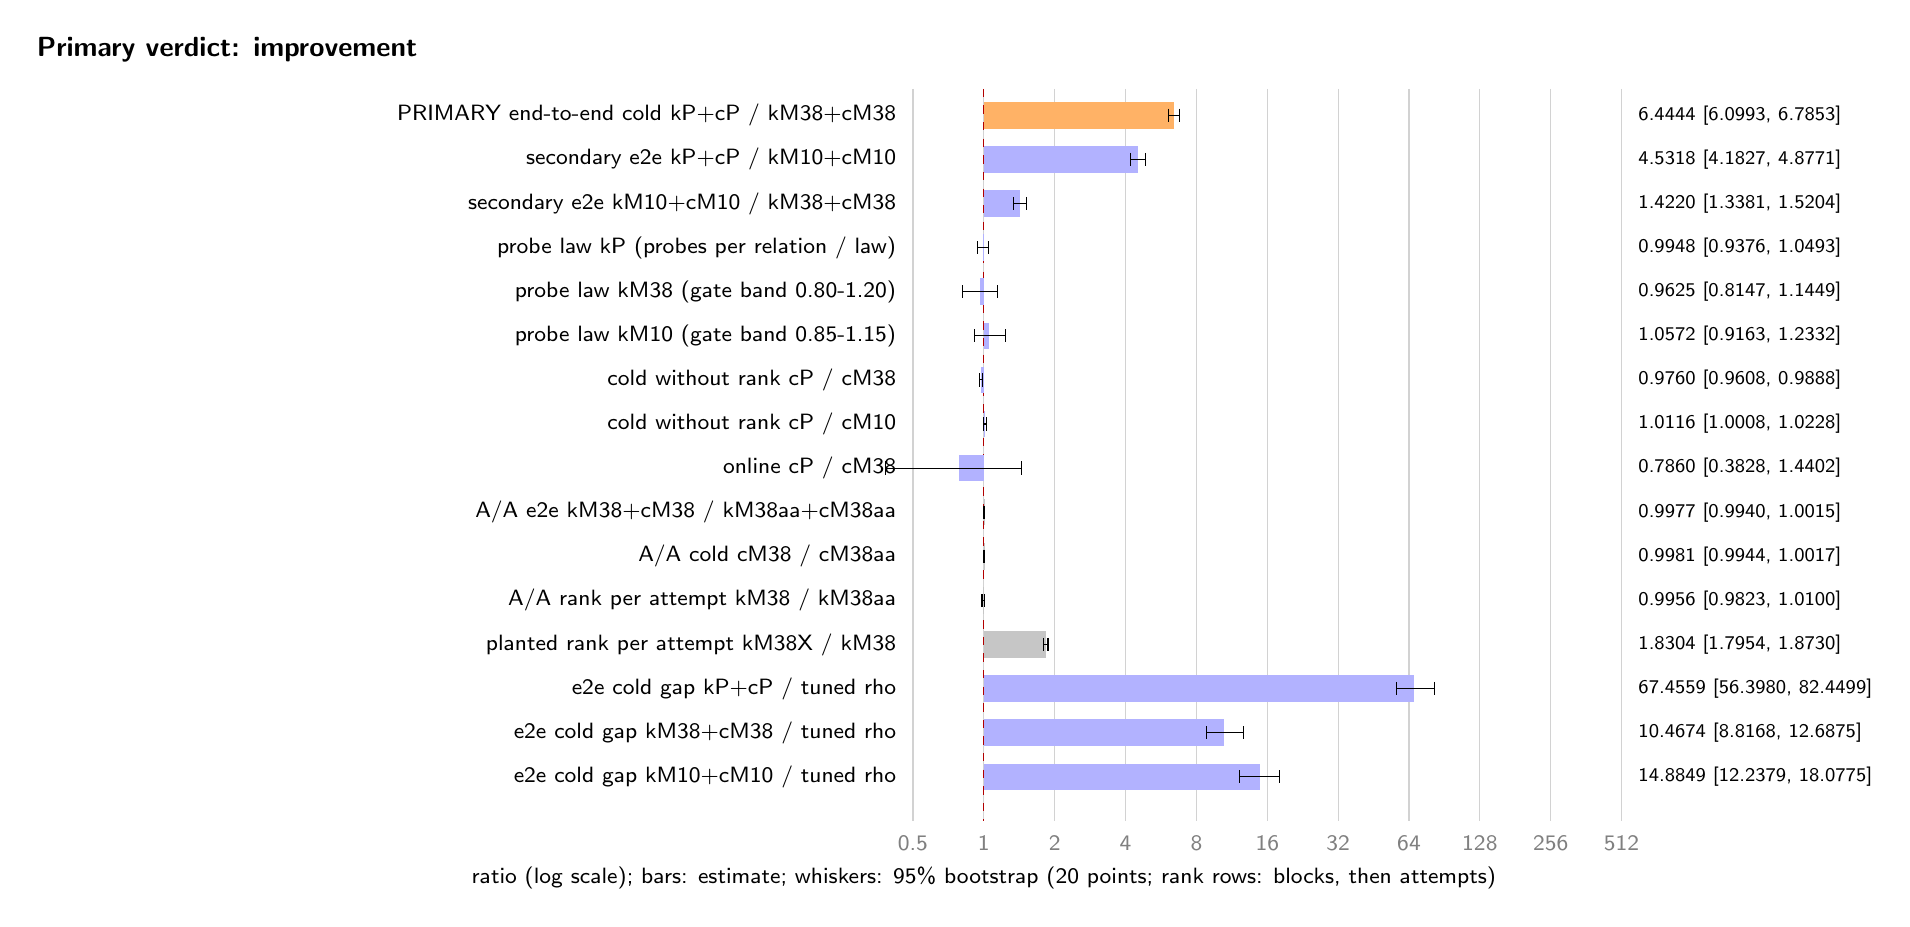
\begin{tikzpicture}[font=\sffamily\footnotesize,x=9mm,y=-5.6mm]
\draw[gray!35] (-1.0000,-0.6) -- (-1.0000,16); \node[gray] at (-1.0000,16.5) {0.5};
\draw[gray!35] (0.0000,-0.6) -- (0.0000,16); \node[gray] at (0.0000,16.5) {1};
\draw[gray!35] (1.0000,-0.6) -- (1.0000,16); \node[gray] at (1.0000,16.5) {2};
\draw[gray!35] (2.0000,-0.6) -- (2.0000,16); \node[gray] at (2.0000,16.5) {4};
\draw[gray!35] (3.0000,-0.6) -- (3.0000,16); \node[gray] at (3.0000,16.5) {8};
\draw[gray!35] (4.0000,-0.6) -- (4.0000,16); \node[gray] at (4.0000,16.5) {16};
\draw[gray!35] (5.0000,-0.6) -- (5.0000,16); \node[gray] at (5.0000,16.5) {32};
\draw[gray!35] (6.0000,-0.6) -- (6.0000,16); \node[gray] at (6.0000,16.5) {64};
\draw[gray!35] (7.0000,-0.6) -- (7.0000,16); \node[gray] at (7.0000,16.5) {128};
\draw[gray!35] (8.0000,-0.6) -- (8.0000,16); \node[gray] at (8.0000,16.5) {256};
\draw[gray!35] (9.0000,-0.6) -- (9.0000,16); \node[gray] at (9.0000,16.5) {512};
\draw[red!70!black,dashed] (0,-0.6) -- (0,16);
\node at (0,17.3) {ratio (log scale); bars: estimate; whiskers: 95\% bootstrap (20 points; rank rows: blocks, then attempts)};
\node[anchor=west,font=\sffamily\bfseries] at (-13.5,-1.5) {Primary verdict: improvement};
\node[anchor=east] at (-1.1000,0) {PRIMARY end-to-end cold kP+cP / kM38+cM38};
\fill[orange!60] (0,-0.300000) rectangle (2.6880,0.300000);
\draw (2.6086,0) -- (2.7624,0); \draw (2.6086,-0.150000) -- (2.6086,0.150000); \draw (2.7624,-0.150000) -- (2.7624,0.150000);
\node[anchor=west,font=\sffamily\scriptsize] at (9.1000,0) {6.4444 [6.0993, 6.7853]};
\node[anchor=east] at (-1.1000,1) {secondary e2e kP+cP / kM10+cM10};
\fill[blue!30] (0,0.700000) rectangle (2.1801,1.300000);
\draw (2.0644,1) -- (2.2860,1); \draw (2.0644,0.850000) -- (2.0644,1.150000); \draw (2.2860,0.850000) -- (2.2860,1.150000);
\node[anchor=west,font=\sffamily\scriptsize] at (9.1000,1) {4.5318 [4.1827, 4.8771]};
\node[anchor=east] at (-1.1000,2) {secondary e2e kM10+cM10 / kM38+cM38};
\fill[blue!30] (0,1.700000) rectangle (0.5079,2.300000);
\draw (0.4202,2) -- (0.6045,2); \draw (0.4202,1.850000) -- (0.4202,2.150000); \draw (0.6045,1.850000) -- (0.6045,2.150000);
\node[anchor=west,font=\sffamily\scriptsize] at (9.1000,2) {1.4220 [1.3381, 1.5204]};
\node[anchor=east] at (-1.1000,3) {probe law kP (probes per relation / law)};
\fill[blue!30] (0,2.700000) rectangle (-0.0075,3.300000);
\draw (-0.0930,3) -- (0.0694,3); \draw (-0.0930,2.850000) -- (-0.0930,3.150000); \draw (0.0694,2.850000) -- (0.0694,3.150000);
\node[anchor=west,font=\sffamily\scriptsize] at (9.1000,3) {0.9948 [0.9376, 1.0493]};
\node[anchor=east] at (-1.1000,4) {probe law kM38 (gate band 0.80-1.20)};
\fill[blue!30] (0,3.700000) rectangle (-0.0552,4.300000);
\draw (-0.2956,4) -- (0.1953,4); \draw (-0.2956,3.850000) -- (-0.2956,4.150000); \draw (0.1953,3.850000) -- (0.1953,4.150000);
\node[anchor=west,font=\sffamily\scriptsize] at (9.1000,4) {0.9625 [0.8147, 1.1449]};
\node[anchor=east] at (-1.1000,5) {probe law kM10 (gate band 0.85-1.15)};
\fill[blue!30] (0,4.700000) rectangle (0.0802,5.300000);
\draw (-0.1261,5) -- (0.3025,5); \draw (-0.1261,4.850000) -- (-0.1261,5.150000); \draw (0.3025,4.850000) -- (0.3025,5.150000);
\node[anchor=west,font=\sffamily\scriptsize] at (9.1000,5) {1.0572 [0.9163, 1.2332]};
\node[anchor=east] at (-1.1000,6) {cold without rank cP / cM38};
\fill[blue!30] (0,5.700000) rectangle (-0.0350,6.300000);
\draw (-0.0577,6) -- (-0.0162,6); \draw (-0.0577,5.850000) -- (-0.0577,6.150000); \draw (-0.0162,5.850000) -- (-0.0162,6.150000);
\node[anchor=west,font=\sffamily\scriptsize] at (9.1000,6) {0.9760 [0.9608, 0.9888]};
\node[anchor=east] at (-1.1000,7) {cold without rank cP / cM10};
\fill[blue!30] (0,6.700000) rectangle (0.0167,7.300000);
\draw (0.0012,7) -- (0.0325,7); \draw (0.0012,6.850000) -- (0.0012,7.150000); \draw (0.0325,6.850000) -- (0.0325,7.150000);
\node[anchor=west,font=\sffamily\scriptsize] at (9.1000,7) {1.0116 [1.0008, 1.0228]};
\node[anchor=east] at (-1.1000,8) {online cP / cM38};
\fill[blue!30] (0,7.700000) rectangle (-0.3473,8.300000);
\draw (-1.3853,8) -- (0.5262,8); \draw (-1.3853,7.850000) -- (-1.3853,8.150000); \draw (0.5262,7.850000) -- (0.5262,8.150000);
\node[anchor=west,font=\sffamily\scriptsize] at (9.1000,8) {0.7860 [0.3828, 1.4402]};
\node[anchor=east] at (-1.1000,9) {A/A e2e kM38+cM38 / kM38aa+cM38aa};
\fill[gray!45] (0,8.700000) rectangle (-0.0033,9.300000);
\draw (-0.0087,9) -- (0.0022,9); \draw (-0.0087,8.850000) -- (-0.0087,9.150000); \draw (0.0022,8.850000) -- (0.0022,9.150000);
\node[anchor=west,font=\sffamily\scriptsize] at (9.1000,9) {0.9977 [0.9940, 1.0015]};
\node[anchor=east] at (-1.1000,10) {A/A cold cM38 / cM38aa};
\fill[gray!45] (0,9.700000) rectangle (-0.0028,10.300000);
\draw (-0.0081,10) -- (0.0025,10); \draw (-0.0081,9.850000) -- (-0.0081,10.150000); \draw (0.0025,9.850000) -- (0.0025,10.150000);
\node[anchor=west,font=\sffamily\scriptsize] at (9.1000,10) {0.9981 [0.9944, 1.0017]};
\node[anchor=east] at (-1.1000,11) {A/A rank per attempt kM38 / kM38aa};
\fill[gray!45] (0,10.700000) rectangle (-0.0063,11.300000);
\draw (-0.0257,11) -- (0.0144,11); \draw (-0.0257,10.850000) -- (-0.0257,11.150000); \draw (0.0144,10.850000) -- (0.0144,11.150000);
\node[anchor=west,font=\sffamily\scriptsize] at (9.1000,11) {0.9956 [0.9823, 1.0100]};
\node[anchor=east] at (-1.1000,12) {planted rank per attempt kM38X / kM38};
\fill[gray!45] (0,11.700000) rectangle (0.8721,12.300000);
\draw (0.8443,12) -- (0.9054,12); \draw (0.8443,11.850000) -- (0.8443,12.150000); \draw (0.9054,11.850000) -- (0.9054,12.150000);
\node[anchor=west,font=\sffamily\scriptsize] at (9.1000,12) {1.8304 [1.7954, 1.8730]};
\node[anchor=east] at (-1.1000,13) {e2e cold gap kP+cP / tuned rho};
\fill[blue!30] (0,12.700000) rectangle (6.0759,13.300000);
\draw (5.8176,13) -- (6.3654,13); \draw (5.8176,12.850000) -- (5.8176,13.150000); \draw (6.3654,12.850000) -- (6.3654,13.150000);
\node[anchor=west,font=\sffamily\scriptsize] at (9.1000,13) {67.4559 [56.3980, 82.4499]};
\node[anchor=east] at (-1.1000,14) {e2e cold gap kM38+cM38 / tuned rho};
\fill[blue!30] (0,13.700000) rectangle (3.3878,14.300000);
\draw (3.1402,14) -- (3.6653,14); \draw (3.1402,13.850000) -- (3.1402,14.150000); \draw (3.6653,13.850000) -- (3.6653,14.150000);
\node[anchor=west,font=\sffamily\scriptsize] at (9.1000,14) {10.4674 [8.8168, 12.6875]};
\node[anchor=east] at (-1.1000,15) {e2e cold gap kM10+cM10 / tuned rho};
\fill[blue!30] (0,14.700000) rectangle (3.8958,15.300000);
\draw (3.6133,15) -- (4.1761,15); \draw (3.6133,14.850000) -- (3.6133,15.150000); \draw (4.1761,14.850000) -- (4.1761,15.150000);
\node[anchor=west,font=\sffamily\scriptsize] at (9.1000,15) {14.8849 [12.2379, 18.0775]};
\end{tikzpicture}
\end{document}
